\documentclass[9pt]{beamer}

\usepackage[english]{babel}
\usepackage[utf8]{inputenc}
\usepackage{hyperref}
\usepackage{verbatim}
\usepackage{pifont}
\usepackage{wasysym}
\usepackage{beamerthemefemto}
\usepackage{multicol}

\definecolor{mygreen}{RGB}{27,156,16}
\definecolor{myred}{RGB}{221,0,17}
\newcommand{\lighter}[1]{{\color{gray} #1}}
\newcommand{\green}[1]{{\color{mygreen} #1}}
\newcommand{\red}[1]{{\color{myred} #1}}

\newcommand{\code}[1]{\texttt{#1}}
\newcommand{\outline}[0]{
  \frame{\frametitle{Outline}\tableofcontents[hideallsubsections]}
}
\newcommand{\outlinereminder}[0]{
  \frame{\frametitle{Outline}
  \tableofcontents[currentsection,subsectionstyle=show/show/hide]}
}

\title[A Constraint Solver for PHP Arrays]{A Constraint Solver for PHP Arrays}
\author[\textbf{I. Enderlin}, A. Giorgetti, F. Bouquet]{
    \textbf{Ivan~Enderlin}\footnote{Funded by Squash},
    Alain~Giorgetti,
    Fabrice~Bouquet
}
\date{
    March 22th, 2013 \\
    CSTVA, Luxembourg
}


\begin{document}

\maketitle

\section{Introduction}

\begin{frame}
\frametitle{Context}

\begin{block}{Web}
\begin{itemize}
\item Many mixed technologies
\item Strings and arrays are the most used and manipulated data
\item They can be complex
\end{itemize}
\end{block}

\begin{block}{PHP}
\begin{itemize}
\item Language that powers more than 75\% of the Web
\item No tool for automatic unit tests generation
\item Highly dynamic: no type
\item Interpreted: source code always available
\end{itemize}
\end{block}

\end{frame}

\begin{frame}
\frametitle{Contract-Driven Testing}

\begin{block}{Principle}
Exploits contracts for test purposes:
\begin{itemize}
\item uses preconditions to generate test data
\item uses postconditions and invariants to establish test verdict by runtime
assertion
checking
\end{itemize}
\end{block}

\begin{block}{Contracts}
\begin{itemize}
\item Invented by B. Meyer in 1992 with Eiffel language
\item Describe a model using annotations
\item Express formal constraints: pre-, postconditions and invariants
\item Can be included directly in the source code applied to:
  \begin{itemize}
  \item classes attributes
  \item methods arguments
  \end{itemize}
\end{itemize}
\end{block}

\end{frame}

\begin{frame}
\frametitle{Design-by-Contract}

\begin{block}{Semantics of contracts}
\begin{itemize}
\item Contractual agreement:
  \begin{itemize}
  \item caller commits to satisfy the pre-condition
  \item callee commits to establish its post-condition
  \end{itemize}
\item Invariants must be satisfied before and after the execution of the methods
\end{itemize}
\end{block}


\begin{block}{Issue of contracts}
\begin{itemize}
\item often expressed with logic formulæ
\item hard to generate data
\end{itemize}
\end{block}

\end{frame}

\begin{frame}
\frametitle{Previous works}

\begin{block}{Praspel, a Specification Language for Contract-Based Testing
(ICTSS'11)}
\begin{itemize}
\item Realistic domains
  \begin{itemize}
  \item structures to automate the validation and the generation of test data
  \end{itemize}
\item Praspel, a new specification language
  \begin{itemize}
  \item adopts Design-by-Contract paradigm
  \item based on realistic domains
  \item implementation in PHP for PHP
  \end{itemize}
\item Automated unit test generator: Praspel tool
  \begin{itemize}
  \item uses Praspel to perform Contract-Driven Testing
  \end{itemize}
\end{itemize}
\end{block}

\begin{block}{Grammar-Based Testing using Realistic Domains (A-MOST'12)}
\begin{itemize}
\item Representing and generating complex textual data with grammar
\item Grammar-based testing in Praspel
\begin{itemize}
\item PP, a new grammar description language
\item two new realistic domains: \code{grammar()} and \code{regex()}
\end{itemize}
\end{itemize}
\end{block}

\end{frame}

\begin{frame}
\frametitle{Motivations and contributions}

\begin{block}{Arrays}
\begin{itemize}
\item Representing and generating PHP arrays
\item PHP arrays cover most of the needs for collections:
\begin{itemize}
\item store key-value pairs of any kinds (hashmap)
\item no specific length or depth
\item efficiently implemented
\end{itemize}
\end{itemize}
\end{block}

\begin{block}{Contributions}
\begin{itemize}
\item Study to known the most popular constraints on PHP arrays
\item Formalize these constraints
\item A constraint solver implemented in PHP
\end{itemize}
\end{block}

\end{frame}

\outline

\section[Praspel]{Realistic domains and Praspel}

\outlinereminder

\begin{frame}
\frametitle{About realistic domains}

\begin{block}{Definition and goal}
\begin{itemize}
\item Are intended to be used for test generation purposes
\item Specify a set of relevant values that can be assigned to a data for a
specific context in a given program
\item Provide features for the validation and generation of data values
\end{itemize}
\end{block}

\begin{block}{Two important features}
\begin{itemize}
\item \textbf{Predicability}, checks if a value belongs to the realistic domain
\item \textbf{Samplability}, generates values that belong to the realistic
domain
\end{itemize}
\end{block}
The sampler can be of many kinds: a random generator, an iterator…
Features are user-defined

\end{frame}

\begin{frame}
\frametitle{Inheritance and interfaces}

\begin{block}{Inheritance}
Since realistic domains are implemented in PHP as classes, they can:
\begin{itemize}
\item inherit from each other
\item refine inherited features of the parent
\item describe a hierarchical universe
\end{itemize}
\end{block}

\begin{block}{Interfaces}
Some realistic domains implement interfaces which characterize them:
\begin{itemize}
\item \code{Constant}, immutable realistic domain with one value (\code{42},
\code{true}, etc.)
\item \code{Interval}, interval with a lower and an upper bound
\item \code{Nonconvex}, discreditable values, i.e. specify a value that no
longer belongs to a realistic domains and should therefore not be generated
\item \code{Finite}, count the number of values
\item \code{Enumerable}, iterate over all the values
\end{itemize}
\end{block}

\end{frame}

\begin{frame}[fragile]
\frametitle{PHP Realistic Annotation and SPEcification Language}

\begin{exampleblock}{Annotated class}
\footnotesize
\only<1>{
\texttt{class C \{} \\
\\
\mbox{\texttt{~~~~/**}} \\
\mbox{\texttt{~~~~~* @invariant foo: float();}} \\
\mbox{\texttt{~~~~~*/}} \\
\mbox{\texttt{~~~~protected \$foo = 0;}} \\
\\
\mbox{\texttt{~~~~/**}} \\
\mbox{\texttt{~~~~~* @requires x: integer() or string('a', 'z', 1);}} \\
\mbox{\texttt{~~~~~* @ensures $\backslash$result: boolean();}} \\
\mbox{\texttt{~~~~~*/}} \\
\mbox{\texttt{~~~~public function f ( \$x ) \{ $\dots$ \}}} \\
\texttt{\}}
}

\only<2>{
\texttt{class C \{} \\
\\
\mbox{\texttt{~~~~/**}} \\
\mbox{\texttt{~~~~~* \red{@invariant foo: float();}}} \\
\mbox{\texttt{~~~~~*/}} \\
\mbox{\texttt{~~~~protected \$foo = 0;}} \\
\\
\mbox{\texttt{~~~~/**}} \\
\mbox{\texttt{~~~~~* @requires x: integer() or string('a', 'z', 1);}} \\
\mbox{\texttt{~~~~~* @ensures $\backslash$result: boolean();}} \\
\mbox{\texttt{~~~~~*/}} \\
\mbox{\texttt{~~~~public function f ( \$x ) \{ $\dots$ \}}} \\
\texttt{\}}
}

\only<3>{
\texttt{class C \{} \\
\\
\mbox{\texttt{~~~~/**}} \\
\mbox{\texttt{~~~~~* @invariant foo: float();}} \\
\mbox{\texttt{~~~~~*/}} \\
\mbox{\texttt{~~~~protected \$foo = 0;}} \\
\\
\mbox{\texttt{~~~~/**}} \\
\mbox{\texttt{~~~~~* \red{@requires x: integer() or string('a', 'z', 1);}}} \\
\mbox{\texttt{~~~~~* @ensures $\backslash$result: boolean();}} \\
\mbox{\texttt{~~~~~*/}} \\
\mbox{\texttt{~~~~public function f ( \red{\$x} ) \{ $\dots$ \}}} \\
\texttt{\}}
}

\only<4>{
\texttt{class C \{} \\
\\
\mbox{\texttt{~~~~/**}} \\
\mbox{\texttt{~~~~~* @invariant foo: float();}} \\
\mbox{\texttt{~~~~~*/}} \\
\mbox{\texttt{~~~~protected \$foo = 0;}} \\
\\
\mbox{\texttt{~~~~/**}} \\
\mbox{\texttt{~~~~~* @requires x: integer() or string('a', 'z', 1);}} \\
\mbox{\texttt{~~~~~* \red{@ensures $\backslash$result: boolean();}}} \\
\mbox{\texttt{~~~~~*/}} \\
\mbox{\texttt{~~~~public function f ( \$x ) \{ $\dots$ \}}} \\
\texttt{\}}
}

\only<5>{
\texttt{class C \{} \\
\\
\mbox{\texttt{~~~~/**}} \\
\mbox{\texttt{~~~~~* @invariant foo: float();}} \\
\mbox{\texttt{~~~~~*/}} \\
\mbox{\texttt{~~~~protected \$foo = 0;}} \\
\\
\mbox{\texttt{~~~~/**}} \\
\mbox{\texttt{~~~~~* @requires x: integer() or string(\red{'a'}, \red{'z'}, \red{1});}} \\
\mbox{\texttt{~~~~~* @ensures $\backslash$result: boolean();}} \\
\mbox{\texttt{~~~~~*/}} \\
\mbox{\texttt{~~~~public function f ( \$x ) \{ $\dots$ \}}} \\
\texttt{\}}
}
\end{exampleblock}

\only<1>{
Expresses contracts using formal constraints, called clauses.
}

\only<2>{
\code{@invariant}: class invariant on class attributes
}

\only<3>{
\code{@requires}: method precondition on class attributes and method arguments
}

\only<4>{
\code{@ensures}: method postcondition on class attributes, and method arguments
and result
}

\only<5>{
Realistic domains can receive parameters: it helps generating structured data
such as arrays, objects, graphs, automata, etc.
}

\end{frame}

\section[Arrays]{Arrays in PHP and Praspel}

\outlinereminder

\begin{frame}
\frametitle{Arrays in PHP}

\begin{block}{Associative array}
An array is always an associative array, a collection of key-value pairs:
\begin{itemize}
\item keys appear at most once
\item keys are reduced to null, integers or strings
%\item keys can be auto-incremented by adding 1 to the last integer index
%starting by 0
\item values can be of many kinds
\end{itemize}
\end{block}

\begin{block}{Content}
\begin{itemize}
\item homogeneous: all keys have the same type, idem for values
\item heterogeneous: keys and values can have distinct types
\end{itemize}
\end{block}

\begin{block}{Length}
The array length (or size) is its number of elements:
\begin{itemize}
\item no predefined length
\item stored internally by the PHP engine
\item can be retrieved with the PHP function \code{count()}
\end{itemize}
\end{block}

\end{frame}

\begin{frame}[fragile]
\frametitle{Arrays in Praspel}

$$\code{array($D$, $L$)}$$
\vspace{-1.5em}
\begin{itemize}
\item $D$, a comma-separated list, between \code{[} and \code{]}, of
{\em array descriptions} of the form \code{from $K$ to $V$}
\begin{itemize}
\item $K$ and $V$ are realistic domain disjunctions, respectively for keys and
values
\end{itemize}
\item $L$, a disjunction of realistic domains of non-negative integers
\end{itemize}

\begin{exampleblock}{Examples of array declaration}
\begin{verbatim}
a1: array([to boolean()], 7..42)
a2: array([from  0..5 or 10 to integer()], 7)
a3: array([from  0..10 to boolean(),
           from 20..30 to float()], 7)
a4: array([from  0..10 or 20..30 to boolean() or float()], 7)
\end{verbatim}
\end{exampleblock}

\end{frame}

\begin{frame}[fragile]
\frametitle{Normal form}

Implicit domain:
$$\code{to $T_1$ or $T_2$} \quad\rightarrow\quad \code{from natural(0, 1) to
$T_1$ or $T_2$}$$

Disjunction removal:
\begin{center}
\begin{tabular}{rcl}
\code{from $F_1$ or $F_2$ to $T_1$ or $T_2$}
&
$\rightarrow$
&
\begin{tabular}{l}
\code{from $F_1$ to $T_1$,} \\
\code{from $F_1$ to $T_2$,} \\
\code{from $F_2$ to $T_1$,} \\
\code{from $F_2$ to $T_2$}
\end{tabular}
\end{tabular}
\end{center}

\begin{exampleblock}{\code{a4} in normal form}
\begin{verbatim}
a4: array([from  0..10 or 20..30 to boolean() or float()], 7)
\end{verbatim}
$\quad\quad\quad\downarrow$
\begin{verbatim}
a4: array([from  0..10 to boolean(),
           from  0..10 to float(),
           from 20..30 to boolean(),
           from 20..30 to float()], 7)
\end{verbatim}
\end{exampleblock}

\end{frame}

\begin{frame}
\frametitle{Frequently used array functions}

\vspace{1em}
{
\small
\begin{itemize}
\item selected 61 PHP projects (for their popularity, impact on the industry and
complexity)
\item represent 28~066 files and 5~220~547 lines of code
\item three most used functions are: \code{count()}, \code{in\_array()} and
\code{array\_key\_exists()}
\end{itemize}
}

\begin{center}
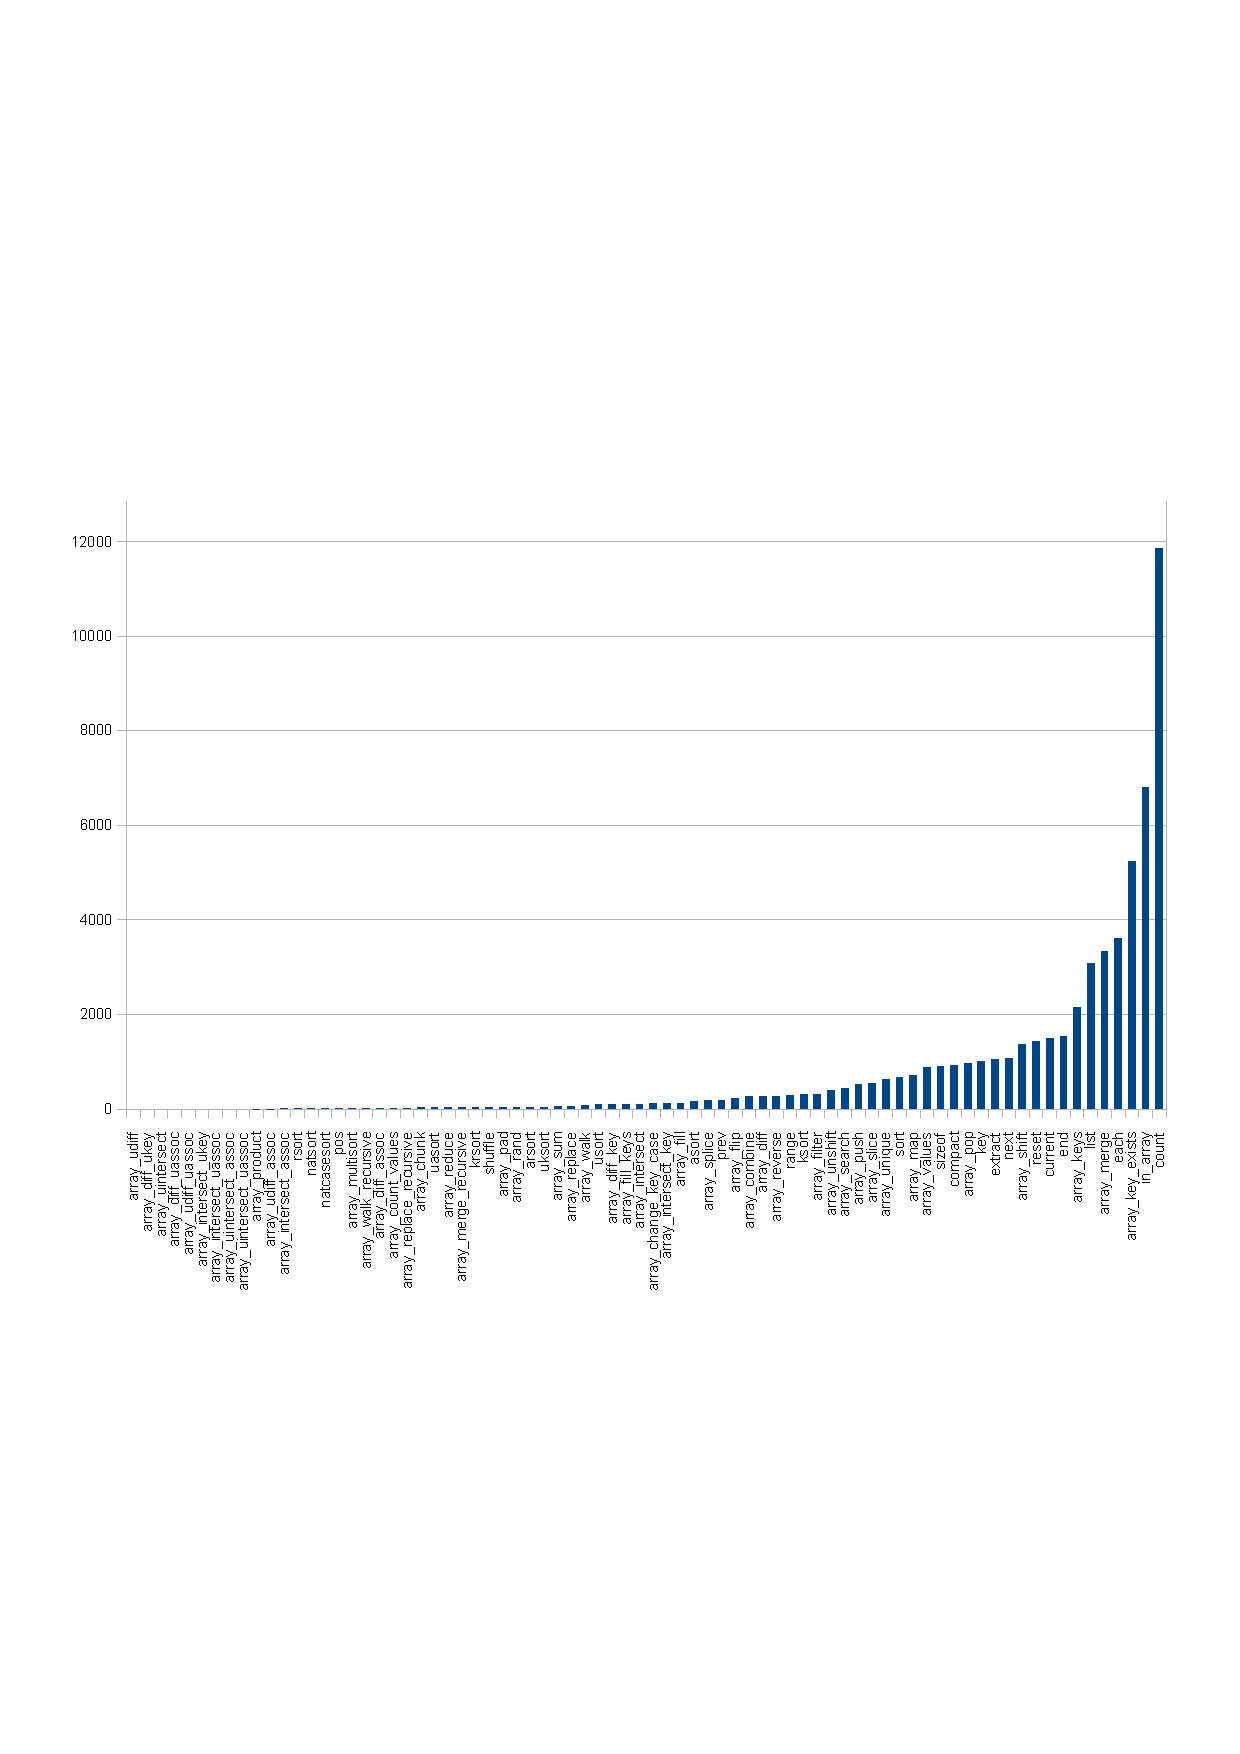
\includegraphics[width=8cm]{Images/Chart.pdf}
\end{center}

\end{frame}

\begin{frame}
\frametitle{Array Conditions}

Extend syntax of declaration with array {\em conditions}:

\begin{block}{Pair condition}
$$\code{a[$K$]:~$V$}$$
\vspace{-1.5em}
\begin{itemize}
\item $K$ and $V$ are realistic domain disjunctions
\item all the keys in $K$ are keys of the array \code{a}
\item all the values associated to keys in $K$ are in $V$
\item $K$ only accepts realistic domains that implements at least the
\code{Constant}, \code{Interval} and \code{Enumerable} interfaces
\item equivalent to use \code{array\_key\_exists()} and \code{in\_array()}
combined
\end{itemize}
\end{block}

% parler des interfaces ici

\end{frame}

\begin{frame}
\frametitle{Array Conditions}

\begin{block}{Key condition}
$$\code{a[$K$]:~\_}$$
\vspace{-1.5em}
\begin{itemize}
\item all the keys from $K$ must be present in the array \code{a}
% plus concret, donner des exemples
\item equivalent to use \code{array\_key\_exists()} with all values in $K$ in
conjunction
\end{itemize}
\end{block}

\begin{block}{Value condition}
$$\code{a[\_]:~$V$}$$
\vspace{-1.5em}
\begin{itemize}
\item all the values in $V$ must be present in the array \code{a}
\item equivalent to use \code{in\_array()} with all values in $V$ in conjunction
\end{itemize}
\end{block}

\end{frame}

\begin{frame}
\frametitle{Array Conditions}

\begin{block}{Pair negation condition}
$$\code{a[$K$]!:~$V$}$$
All the keys in $K$ have a value in the array \code{a}. None of this value is in
$V$.
\end{block}

\begin{block}{Key and value negation condition}
$$\code{a[$K$]!:~\_}$$
No key in $K$ appears in \code{a}.

$$\code{a[\_]!:~$V$}$$
No value in $V$ appears in \code{a}.
\end{block}

\end{frame}

\begin{frame}[fragile]
\frametitle{Array Conditions}

\begin{block}{Unicity of values}
$$\code{a is unique}$$
expresses unicity condition of values. We cannot have the same value twice in
the array \code{a}. \\

{
\small
Reminder: keys are always unique.
}
\end{block}

\begin{exampleblock}{Running example, system = conjunction of array conditions}
\begin{verbatim}
length: 0..5 or 10
a     : array([to string('a', 'e', 1)], length)
a[0]  : 'b' or 'd'
a is unique
\end{verbatim}
% ajouter des instances
\end{exampleblock}

\end{frame}

\section[Solver]{Constraint Solver}

\outlinereminder

\begin{frame}[fragile]
\frametitle{Conditions to constraints}

The solver constructs an array satisfying all the conditions.
$$\code{a: array($D$, $L$)}$$
\vspace{-1.5em}
\begin{itemize}
\item $D$ is \code{[from $F_1$ to $T_1$, $\dots$, from $F_p$ to $T_p$]} with $1
\le p$, in normal form
\item $L$ is \code{$L_1$ or $\dots$ or $L_m$} with $1 \le m$ and are realistic
domains that inherit from the \code{Integer} realistic domain and that are
non-negatives
\end{itemize}

\begin{exampleblock}{Example}
\begin{verbatim}
length: 0..5 or 10
a     : array([to string('a', 'e', 1)], length)
\end{verbatim}
\begin{itemize}
\item $p = 1$ and $m = 2$
\item $L_1 = [\code{0..5}]$ and $L_2 = \{\code{10}\}$
\item $F_1 = \code{natural(0, 1)}$ and $T_1 = \code{string('a', 'e', 1)}$
\end{itemize}
\end{exampleblock}

\end{frame}

\begin{frame}
\frametitle{Variables}

Constraint variables are:
\begin{itemize}
\item array size $S$, which is a non-negative integer
\item sets $X$ and $Y$, which respectively are the array domain (set of
keys) and codomain (set of values)
\item array content $H$, which is a total function from $X$ to $Y$
\item realistic domains $X_1, \dots, X_p$ (resp. $Y_1, \dots, Y_p$), which
are subsets of the realistic domains $F_1, \dots, F_p$ (resp. $T_1, \dots, T_p$)
compatible with all the array conditions
\end{itemize}
Goal: finding a value of $H$, $X_i$ and $Y_i$.

\end{frame}

\begin{frame}[fragile]
\frametitle{Cardinality Constraints}

{
\footnotesize
Let $\mathrm{card}(E)$ denotes the cardinality of the finite set $E$.
}

% faire un tableau, plus simple
% grouper les contraintes entre globales et génériques

\begin{center}
\begin{tabular}{rcll}
$\mathrm{card}(X)$ &    =   & $S$                & $\quad\quad$size is the number of keys \\
$S$                &  $\ge$ & $0$                & $\quad\quad$size is non-negative \\
$\mathrm{card}(X)$ &  $\ge$ & $\mathrm{card}(Y)$ & $\quad\quad$no unicity on values (by default) \\
$\mathrm{card}(X)$ &    =   & $\mathrm{card}(Y)$ & $\quad\quad$\code{a is unique}
\end{tabular}
\end{center}

The array size $S$ should be in one of the sets $L_1, \dots, L_m$, so:
$$S \in L_1 \cup \dots \cup L_m$$

\begin{exampleblock}{Example}
\begin{verbatim}
length: 0..5 or 10
\end{verbatim}
$L_1 \subseteq [\code{0..5}]$ and $L_2 \subseteq \{\code{10}\}$. The size $S$ is
constrained by $S \in L_1 \cup L_2$.
\end{exampleblock}

\end{frame}

\begin{frame}[fragile]
\frametitle{Constraints on Pairs}

{
\footnotesize
When $x \in X$ holds, $H(x) = y$ means that the key-value pair $(x, y)$ is in
the array. We extend $H$ to any subset $E$ of $X$ with $H'$ defined by:
$$H'(E) = \{H(x) \text{ s.t. } x \in E\}$$
}

For each array condition \code{a[$K$]:~$V$}, where $K$ and $V$ are domain
disjunctions, we introduce the constraints:
$$K \subseteq X \quad\quad\quad H'(K) \subseteq V$$

\begin{exampleblock}{Translation of a pair condition}
\begin{verbatim}
a[0]: 'b' or 'd'
\end{verbatim}
$K = \{\code{0}\}$, $V = \{\code{'b'}, \code{'d'}\}$. The constraints are
$\{\code{0}\} \subseteq X$ and $H'(\{\code{0}\}) \subseteq \{\code{'b'},
\code{'d'}\}$.
\end{exampleblock}

\end{frame}

\begin{frame}
\frametitle{Propagation, Consistency and Labelling}

\begin{block}{Propagation and consistency}
\begin{itemize}
\item Propagation uses an AC3 algorithm implemented in PHP
\item All kinds of realistic domains (\code{Constant}, \code{Interval},
\code{Nonconvex}, etc.) have a {\em revise} method to reduce the domain
\item The consistency is checking there is no empty domain for the four
variables $S$, $H$, $X$ and $Y$
\end{itemize}
\end{block}

\begin{block}{Labelling}
Heuristic to converge quickly: chosing a value for the variable $S$ at first.
Then, the solver tries to compute the sets $X$ and $Y$:
\begin{itemize}
\item use a random generator to generate a value in a domain disjunction
\item the generated value is then propagated
\item if an inconsistency is detected, a new constraint is added (if $S = 5$
leads to an inconsistency, we add the constraint $S \neq 5$)
\end{itemize}
When all variables are labelled, the solver returns the solution.
\end{block}

\end{frame}

\section{Experimentation}

\outlinereminder

\begin{frame}
\frametitle{Evaluate the solver efficiency}

Its capability to avoid or reduce rejection when generating data from systems
(i.e. conjunction of array conditions).

Measures:
\begin{itemize}
\item the number of backtracks in the solver
\item the time to generate data from satisfiable systems
\item how many unsatisfiable systems are detected
\end{itemize}

\begin{block}{Process}
The experimentation is composed of three steps:
\begin{itemize}
\item system generation
\item data generation (i.e. system solving)
\item measuring step
\end{itemize}
We generate systems on arrays containing strings and integers, and of length 5
to 20.
\end{block}

\end{frame}

\begin{frame}
\frametitle{System and data generation}

\begin{block}{System generation}
\begin{itemize}
\item Use the Praspel grammar, including array conditions
\item Apply previous work on grammar-based testing
\item Use the bounded-exhaustive generation algorithm:
\begin{itemize}
\item lot of data
\item all branches are covered
\item all tokens are covered
\end{itemize}
\end{itemize}
\end{block}

\begin{block}{Data generation}
\begin{itemize}
\item Call the solver on each produced system to generate an array satisfying
it.
\item Every generated array is evaluated by the predicability feature associated
to the system of array conditions, to check the solver soundness.
\end{itemize}
\end{block}

\end{frame}

\begin{frame}
\frametitle{Measures}

During data generation:
\begin{itemize}
\item count only the array generation time
\item measure the number of backtracks in the solver
\item measure the number of rejected systems
\end{itemize}

\vspace{1em}
\begin{center}
\footnotesize
\begin{tabular}{|c|c|c|c|c|c|}
\hline
$n$ & generated & backtracks & backtracks per & rejected & generation \\
    & systems   &            & system         & systems  & time (ms)  \\
\hline
 10 &        14 &          0 &              0 &        0 &      6.484 \\
 15 &        86 &         34 &           0.40 &        0 &     42.167 \\
 18 &       210 &         91 &           0.43 &        0 &    141.694 \\
 19 &       275 &        103 &           0.37 &        0 &    229.001 \\
 20 &       492 &        114 &           0.23 &        0 &    372.241 \\
% 22
% 25
\hline
\end{tabular}
\end{center}

\end{frame}

\section{Conclusion}

\begin{frame}
\frametitle{What have we seen?}

\begin{itemize}
\item An extension of the Praspel language to specify usual conditions on PHP
arrays
\item Semantics of conditions expressed by constraints
\item Designed and implemented a constraint solver in PHP to generate test data
\begin{itemize}
%\item uses a random generator to ensure a diversity of generated solutions
\item integrated in realistic domains
\item can be used within the Praspel framework
\end{itemize}
\item Rejection has been totally removed
\end{itemize}

\end{frame}

\begin{frame}
\frametitle{Future works}

\begin{itemize}
\item Extend the experimentation:
\begin{itemize}
\item generate inconsistencies and observe the solver behavior
\end{itemize}
\item Formalize more constraints and extend the solver
\item Transform constraints into the formalism of MiniZinc:
\begin{itemize}
\item compare to other solvers regarding performances and capabilities to find
solutions
\end{itemize}
\item Extend solver to strings (because a string is an array of characters)
\end{itemize}

\end{frame}

\begin{frame}
\frametitle{Thanks!}

\begin{center}
Thank you for your attention! Any questions?
\end{center}

\end{frame}

\begin{frame}
\frametitle{References}

\bibliographystyle{amsalpha}
\bibliography{Bibliography}
\nocite{EnderlinDGO11,EnderlinDGB12}
\end{frame}

\end{document}
